\section{ECG噪声检测与分类方法}
在这部分中,我们提出了一种简单直接的方法来检测和分类ECG噪声。这种方法由四部分组成:信号抑制及噪声增强,特征提取,振幅检测,还有基于决策树的噪声分类。

\subsection{信号抑制和噪声增强}

\begin{wrapfigure}{l}{22em}%靠文字内容的左侧
\label{figNo.2}
\setlength{\belowcaptionskip}{-10pt}
\setlength{\abovecaptionskip}{5pt}
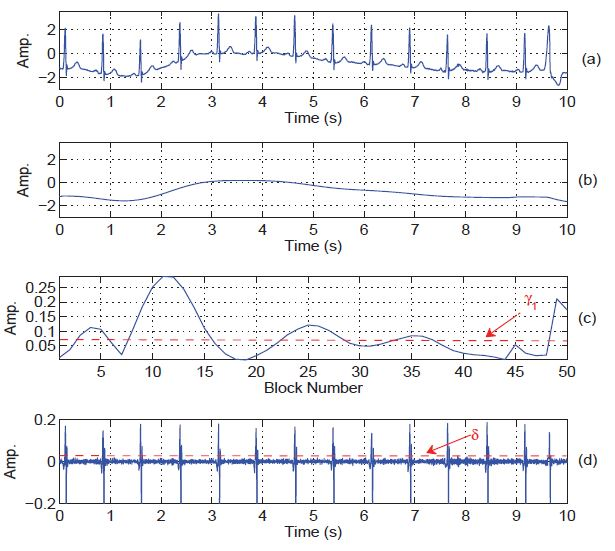
\includegraphics[width=0.55\columnwidth]{fig2.jpg}
\caption{
\wuhao
从带BW噪声ECG信号中获取的特征信号。(a)为受干扰ECG信号,(b)为提取得到的带BW噪声低频组分,(c)为动态振幅范围估计,(d)为高频组分。
}
\end{wrapfigure}
\song
该过程中,我们提出的方法使用了滑动平均滤波器来提取低频噪声组分(包含BW噪声)和高频噪声组分(包括PLI噪声,MA噪声和记录设备噪声)。滤波步骤处理了10s的ECG信号$x[n]$。用于将输入ECG信号中BW噪声(或低频噪声伪影)提取出来的滑动平均滤波器可表示如下:
\begin{equation}
  \mathbf{u}[n]=\frac{1}{L+1}\sum^{L}_{k=0}\mathbf{x}[n-k]
  \label{equ1}
\end{equation}
这里L表示滑动平均滤波器的长度。该过程中,选取这样的滤波器长度是为了让其足以捕捉到0.5Hz以下的BW噪声。同时,用于将输入ECG信号中的高频噪声(包括PLI噪声,MA噪声以及记录设备噪声)提取出来的滤波器差分方程如下:
\begin{equation}
  \mathrm{v_{1}}[n]=\frac{1}{L+1}\sum^{L}_{k=0}\mathbf{x}[n-k]
  \label{equ2}
\end{equation}

\begin{equation}
  \mathrm{v}[n]=\mathrm{x}[n]-\mathrm{v_{1}}[n],~~n=0,1,2......,N-1 
\label{equ3}
\end{equation}

第二个滑动平均滤波器长度的选取依据是令其足以捕捉40Hz以下的ECG信号。为了避免相位滞后,滤波操作采用了零相位滤波器(滤波器系数为$b_{k}=1,~~k=0,1,2,3......,L-1$)。之后,通过检测BW,PLI,MA以及记录设备噪声的出现来提取低频组分和高频组分中的噪声信号特征。图2(b)及(d)中的输出波形展示了从带噪ECG信号中获取的低频和高频组分。\\

\subsection{特征提取}
特征提取通过以下两个步骤实现:非重叠分帧和特征计算。在分帧过程中,经过滤波的信号被分为了非重叠的帧,帧长200ms。在这个过程中,信号$\mathbf{u}[n]$中第$k$帧$\mathbf{u}_{k}[n]$由以下算式给出:
\begin{equation}
  \mathbf{u}_{k}[n]=\mathbf{u}[\mathrm{P}k+n]~~n=1,2,...\mathrm{P}
  \label{equ4}
\end{equation}
此处$k=0,1...\mathrm{M}-1,\mathrm{M}=\lfloor\mathrm{\frac{N}{P}}\rfloor$,P表示帧长。通过计算每帧中振幅的最大最小值来鉴别出掩盖了PQRST波形中低振幅局域波的背景噪声。该过程中,每帧中的最大最小振幅值由如下算式计算得出:
\begin{equation}
\begin{aligned}
&a_{\max}[k]=\max \{u_{k}[n]\}~~k=0,1,...\mathrm{M-1} \\
&a_{\min}[k]=\min \{u_{k}[n]\}~~k=0,1,...\mathrm{M-1}
\end{aligned}
\label{equ5}
\end{equation}
通过比较每帧信号的动态振幅范围和预设的振幅阈值,BW噪声可以被探测到。动态振幅范围由以下算式给出:
\begin{equation}
a_{\mathrm{dr}}[k]=a_{\max}[k]-a_{\min}[k]~~k=0,1,2,...\mathrm{M}-1
 \label{equ6}
\end{equation}

特征提取中每个步骤的输出波形见图2。图2(b)中的低频组分包含了振幅出现大幅波动的BW噪声。为了将BW噪声和突变伪影区分开来,该方法估算了每帧信号的局部动态振幅范围。低频组分中,对动态振幅范围进行估算后的输出结果如图2(c)。通过设置预设的振幅阈值条件$\gamma_1,a_{\mathrm{dr}}[k]>\gamma_1$,检测得具有较低振幅帧数比率的BW噪声被与突变伪影区分开来。

\begin{table}[htbp]
\scriptsize
\centering
\caption{ECG局部波类型及其特征
\label{tabNo.1}}
\begin{tabular}{|c|c|c|}
\hline 
ECG波类型 & 振幅范围 & 持续时间 \\ 
\hline 
P波 & 0.1-0.2mV & 100ms \\ 
\hline 
QRS波群 & 0.5-1.0mV & 80-100ms \\ 
\hline 
T波 & $\approx0.5\mathrm{mV}$ & 150-200ms \\ 
\hline 
U波 & 1-2mm或T波振幅的25\% & - \\ 
\hline 
\end{tabular} 
\end{table}

对于高频噪声(如PLI和MA噪声)的检测,首先通过公式\ref{equ3}提取信号的高频组分$\mathbf{v}(n)$。滤波器的阶数被设定为能够正确捕获高频组分中50/60Hz的PLI噪声和肌电干扰噪声。以用于测试的含BW噪声ECG信号为处理对象,从中提取的高频组分如图2(d)所示。经观测,高频组分中不仅含有低振幅高频噪声,也含有部分QRS波群信号。在这一步处理过程中,通过比较高频组分振幅的最大绝对值和预设的振幅阈值$\delta$,高频噪声的影响程度得以确定。而该振幅阈值的确定则依赖于ECG信号中局部波形的各项振幅值(见表\ref{tabNo.1})。基于这些局部波振幅值,振幅阈值得以选定。低振幅的PLI噪声和肌电干扰噪声或许能通过一个简单的平滑滤波器去除。该方法假设高振幅值的PLI和肌电干扰噪声能够掩盖住中等振幅值局部波(包括P,Q,T,U波)的关键点(如起始点,终止点和峰值点)。若能使用这种噪声消除技术恢复关键点,则这时的噪声水平被认为是可接受的。振幅阈值$\delta$的选择值为0.02mV。至于高频噪声的探测,我们估算了振幅值大于$\delta=0.02\mathrm{mV}$的采样点的总数($\mathrm{N_{HF}}$)。如果估算的$\mathrm{N_{HF}>2 \times F_s}$,则算法认为存在高频噪声。

一旦确定了高频噪声确实存在,高频噪声将会被进一步分类为PLI噪声和肌电干扰噪声。
\begin{wrapfigure}{r}{24em}%靠文字内容的左侧
\label{figNo.3}
\centering
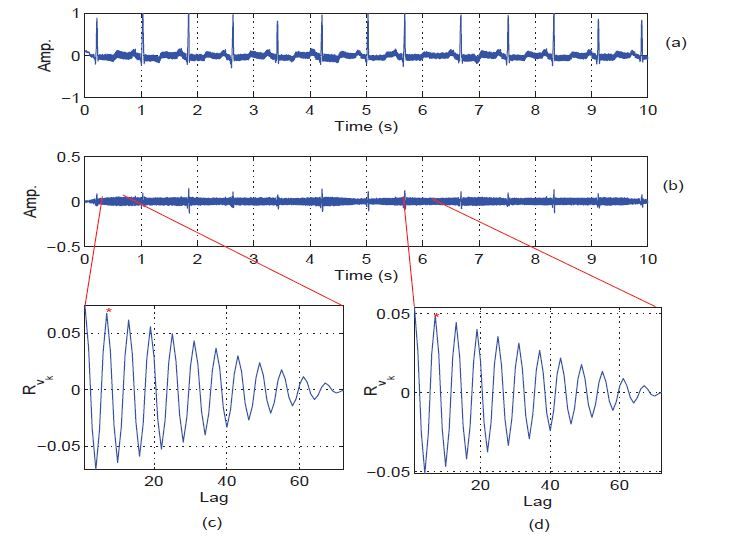
\includegraphics[width=0.5\columnwidth]{fig3.jpg}
\caption{
\wuhao
从带PLI噪声的高频组分中获取的帧信号表消除了周期性。(a)为带PLI噪声的ECG信号,(b)为提取所得带PLI噪声的高频组分仍包含了ECG中的QRS波群高频部分。(c)为第一个R峰与第二个R峰之间的采样帧中的交流信号;(d)为第八个R峰和第九个R峰之间的交流信号。
}
\end{wrapfigure}
在高频噪声分类程序中,高频组分经过了重叠分帧,帧长为200ms,帧移Q为100ms。重叠分帧的方法可表达为:
\begin{equation}
  \mathbf{v}_{k}[n]=\mathbf{v}[\frac{\mathrm{P}k}{2}+n]~~n=1,2,...\mathrm{P}
  \label{equ7}
\end{equation}
其中$k=0,1,...\mathrm{M_1}-1$,且$\mathrm{M_1}=\lfloor\frac{N}{Q}\rfloor$。在本部分处理中,利用自相关性将PLI结构噪声和肌电干扰噪声分离。在我们之前的研究中,使用自相关函数来确定信号的周期被证明是有效的。对于每帧信号$\mathbf{v}_{k}[n]$,自相关序列计算如下:
\begin{equation}
  \mathbf{R}_{k}(\tau)=\frac{1}{P}\sum^{\mathrm{P}}_{n=0}\mathbf{v}_{k}[n]\mathbf{v}_{k}[n+\tau]
  \label{equ8}
\end{equation}
其中$\mathbf{R}_{k}(\tau)$表示$\mathbf{v}_{k}[n]$的自相关函数(Autocorrelation Function, ACF),$\tau$表示自相关函数的延迟时间。通过参考第一个负过零点(由正到负的过零点称为负过零点,译者注),每帧中自相关函数的局部最大值能够被估算出来。图3表示出了自相关函数的结果,以便观察。自相关图谱显示PLI结构噪声是存在的。ACF的有效性也进一步通过处理含有肌电干扰和PLI噪声的ECG信号进行了评估。自相关性提取的输出波形见图4,图5。对于这两个带噪ECG信号,低频组分示意图显示出了振幅值小于振幅阈值$\delta$的BW噪声组分。含PLI与MA噪声的ECG信号高频组分分别见图4(d)和图5(d)。ACF特征信号见图4(e)和图5(e)。从图4(e)的ACF信号中可看出多数帧中,信号的峰值小于0.2。该实验中,我们注意到大多数帧肌电干扰信号的帧内相关性不显著。同时,图5(e)中的ACF结果显示大多数帧中的信号峰值大于0.4。通过选择一个合适的自相关峰阈值,高频组分能够被分为PLI噪声和肌电干扰噪声。一种简单的多级决策噪声检测和分类方法如图6所示。 
\begin{figure}[htbp]
\begin{center}
\begin{minipage}{0.45\linewidth}
\label{figNo.4}
\centering
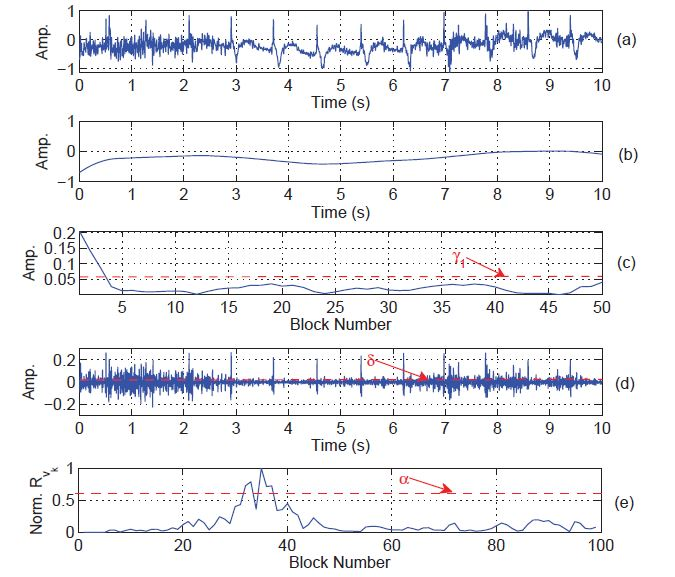
\includegraphics[height=0.8\textwidth]{fig4.jpg}
\caption{\kaishu \xiaowuhao 受肌电干扰的ECG的特征提取。(a)受干扰的ECG;(b)提取出的带BW的低频组分;(c)动态振幅范围估算;(d)高频组分;(e)最大自相关峰方法提取的自相关函数特征。}
\end{minipage}~~
\begin{minipage}{0.45\linewidth}
\label{figNo.5}
\centering
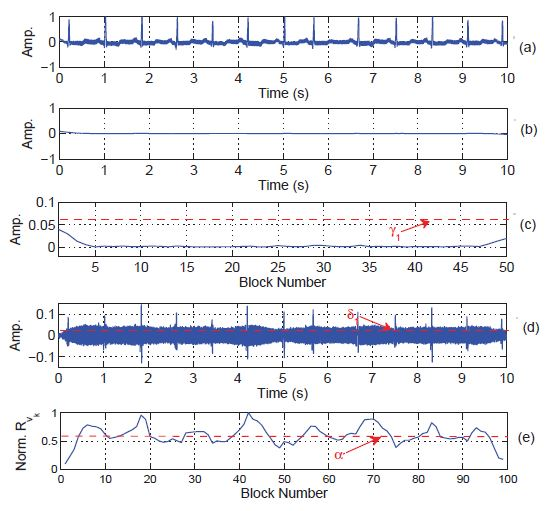
\includegraphics[height=0.8\textwidth]{fig5.jpg}
\caption{\kaishu \xiaowuhao 带PLI噪声ECG的特征提取。(a)受干扰ECG信号;(b)带BW噪声的低频组分;(c)动态振幅范围评估;(d)高频组分;(e)使用最大自相关峰提取的自相关函数特征。}

\end{minipage}
\end{center}
\end{figure}

